\def\year{2021}\relax
% File: LatentVars-aaai.tex

\documentclass[letterpaper]{article}

% DO NOT CHANGE THIS
\usepackage{aaai21} % DO NOT CHANGE THIS
\usepackage{times} % DO NOT CHANGE THIS
\usepackage{helvet} % DO NOT CHANGE THIS
\usepackage{courier} % DO NOT CHANGE THIS
\usepackage[hyphens]{url} % DO NOT CHANGE THIS
\usepackage{graphicx} % DO NOT CHANGE THIS
\urlstyle{rm} % DO NOT CHANGE THIS
\def\UrlFont{\rm} % DO NOT CHANGE THIS
\usepackage{graphicx} % DO NOT CHANGE THIS
\usepackage{natbib}
% DO NOT CHANGE THIS OR ADD OPTIONS
\usepackage{caption}
% DO NOT CHANGE THIS OR ADD OPTIONS
\frenchspacing % DO NOT CHANGE THIS
\setlength{\pdfpagewidth}{8.5in} % DO NOT CHANGE THIS
\setlength{\pdfpageheight}{11in} % DO NOT CHANGE THIS

% THIS IS OUR "EXTRA" SECTION - REVIEW FOR COMPLIANCE WITH AAAI RULES
\usepackage{xr}
\externaldocument[main-]{LatentVars-aaai}

\usepackage[utf8]{inputenc} % allow utf-8 input
\usepackage[T1]{fontenc}    % use 8-bit T1 fonts
\newcommand{\theHalgorithm}{\arabic{algorithm}}

\usepackage{amsthm}

\usepackage{booktabs}       % professional-quality tables
\usepackage{amsfonts}       % blackboard math symbols - THIS MAY CAUSE PROBLEMS
\usepackage{nicefrac}       % compact symbols for 1/2, etc.
\usepackage{microtype}      % microtypography
\usepackage{multirow}				% for multi-row labels
\usepackage{subfig}					% for laying out multi-panel figures and tables 
\usepackage{cancel}					% for crossing out characters
\usepackage{amsmath}				% for splitting multi-line equations
\usepackage{placeins}				% for table and figure positioning
\usepackage{mathtools}			% for \vdotswithin{}
\usepackage{resizegather}   % for gathering multi-lines to one line
%package for graph layout
\usepackage[pdf]{graphviz}	% THIS MAY CAUSE PROBLEMS

\usepackage{algorithm}% http://ctan.org/pkg/algorithms
\usepackage{algpseudocode}% http://ctan.org/pkg/algorithmicx

\externaldocument{LatentVars-aaa}
%
% PDF Info Is REQUIRED.
% For /Author, add all authors within the parentheses,
% separated by commas. No accents or commands.
% For /Title, add Title in Mixed Case.
% No accents or commands. Retain the parentheses.
\pdfinfo{
/Title (Identification of Latent Variables From Graphical Model Residuals)
/Author (Anonymous)
} %Leave this

\title{Identification of Latent Variables From Graphical Model Residuals: Supplementary Material}

\newtheorem{theorem}{Theorem}

\begin{document}

\maketitle

\begin{abstract}
Graph-based causal discovery methods aim to capture conditional independencies consistent with the observed data and differentiate causal relationships from indirect or induced ones.  Successful construction of graphical models of data depends on the assumption of causal sufficiency: that is, that all confounding variables are measured. When this assumption is not met, learned graphical structures may become arbitrarily incorrect and effects implied by such models may be wrongly attributed, carry the wrong magnitude, or mis-represent direction of correlation.  Wide application of graphical models to increasingly less curated "big data" draws renewed attention to the unobserved confounder problem.  

We present a novel method that aims to control for the latent space when estimating a DAG by iteratively deriving proxies for the latent space from the residuals of the inferred model.  Under mild assumptions, our method improves structural inference of gaussian graphical models and enhances identifiability of the causal effect. In addition, when the model is being used to predict outcomes, it un-confounds the coefficients on the parents of the outcomes and leads to improved predictive performance when out-of-sample regime is very different from the training data.  We show that any improvement of prediction of an outcome is intrinsically capped and cannot rise beyond a certain limit as compared to the confounded model.  We extend our methodology beyond GGMs to ordinal variables and nonlinear cases.  Our R package provides both PCA and autoencoder implementations of the methodology, suitable for GGMs with some guarantees and for better performance in general cases but without such guarantees. 
\end{abstract}

\section{Theorems}
\begin{theorem}[Inferrability]
\label{thm:inferrability}
Posit that we know the true DAG $G$ over $D$, but not $U = G_u \setminus G$, the latent space's edges to observed variables.  Assume that $L$ is orthogonal, with no variable in $D$ a parent of any variable in $U$. Define as $R_C = C^{U,G} - \bar{C}^{U,G}$ the residuals of all children of $U$ that also have parents in $G$.  If relationships described by $G$ are linear, we can infer $U$ from $R_C$ up to sign and scale.  

\begin{proof}
Consider $G_u$ (Figure \ref{fig:residualsInGraph}).  Since all variables in $U$ are upstream of $C^{U,G}$, and since all residuals $R_{U,C}$ are downstream of $C^{U,G}$, we can write $U \perp\!\!\!\perp R_C | C^{U,G}$.  Therefore, all paths $U \rightarrow R_C$ have the form $U \rightarrow C^{U,G} \rightarrow R_C$.  Further, $R_i \perp\!\!\!\perp R_j | C_i,C_j,U,   \forall C_i, C_j \in C^{U,G}$. Also, $U_i \perp\!\!\!\perp U_j, \forall i, j \in U$ by definition of orthogonality.  Therefore, no paths exist in $G_u$ within $U$ or within $R$.  Further, with respect to individual residuals (and their immediate parent variables), each $Pa(R_i)$ can be written as a linear combination of parents of $R_i$ by progressive summation upwards from $R_i$, thus collapsing complex paths within $G$ to single meta-nodes.  This logical procedure demonstrates that $U->G->R$ can be viewed as a bipartite graph $U->R$ (Figure \ref{fig:linearizingDagCatchment}).  \cite{anandkumar_learning_2013} showed that, if such a bipartite graph met the expansion property, the latent space of $R$ could be inferred up to sign and scale.  That is, starting with $G$, it is possible to infer $U$, where $G$ is needed to compute $R$.  

To summarize, to detect latent space $U$, we can compute $R^*_C$ when $U$ is unknown and can't be used in estimation - when we only know $G$.   Now, $\exists i, j s.t. R^*_i \not\perp\!\!\!\perp R^*_j | \bar{C}_i, \bar{C}_j$. These collinear (or rank-correlated) residuals contain signal from latent space, as shown earlier.  Thus, it is the violation of independence of residuals  that gives rise to identifiability. 
\end{proof}
\end{theorem}

\begin{figure}[h]
	\centering
	\digraph[scale=0.5]{g3}{
			graph[ranksep=0.1];
      node [shape=circle, style="filled"];
      U1 [fillcolor=red, label=<U<SUB>1</SUB>>];
      V1 [fillcolor=gray, label=<V<SUB>2</SUB>>];
      R1 [fillcolor=white, label=<R<SUB>2</SUB>>, style=dotted];     
      V2 [fillcolor=gray, label=<V<SUB>3</SUB>>];
      R2 [fillcolor=white, label=<R<SUB>3</SUB>>, style=dotted];  
      V3 [fillcolor=gray, label=<V<SUB>4</SUB>>];
      R3 [fillcolor=white, label=<R<SUB>4</SUB>>, style=dotted];  
      V4 [fillcolor=gray, label=<V<SUB>5</SUB>>];
      R4 [fillcolor=white, label=<R<SUB>5</SUB>>, style=dotted];  
      V5 [fillcolor=white, label=<V<SUB>7</SUB>>];
      O1 [fillcolor=green, label=<O<SUB>1</SUB>>];
      RO1 [fillcolor=white, label=<R<SUB>O<SUB>1</SUB></SUB>>, style=dotted];  
      U1 -> V1; U1 -> V2; U1-> V3; U1 -> V4; V3-> O1; V4 -> O1; U1 -> O1; V1 -> V2; V4 -> V5; V5 -> O1; V1 -> R1; V2 -> R2; V3 -> R3; V4 -> R4; O1 -> RO1
	}
	\caption{Residuals $R$ can be calculated from graph $G = G_u \setminus L$ and data $D$.  Residuals of descendants of latent space $L$ will contain its "shadows".  It may be helpful to view them as leaf nodes in some contexts.}
	\label{fig:residualsInGraph}
\end{figure}

\begin{figure}[h]
	\centering
	\digraph[scale=0.5]{g4}{
			graph[ranksep=0.1];
      node [shape=circle, style="filled"];
      G1U1 [fillcolor=red, label=<U<SUB>1</SUB>>]; 
      G1Ell1 [fillcolor=red, label="..."];
      G1U2 [fillcolor=red, label=<U<SUB>2</SUB>>];
      G1Uk [fillcolor=red, label=<U<SUB>k</SUB>>];
      G1G1 [fillcolor=gray, label=<G<SUB>1</SUB>>];
      G1G2 [fillcolor=gray, label=<G<SUB>2</SUB>>];
      G1Ell2 [fillcolor=gray, label="..."];
      G1Gi [fillcolor=gray, label=<G<SUB>i</SUB>>];
      G1Gj [fillcolor=gray, label=<G<SUB>j</SUB>>];
	  G1Gk [fillcolor=gray, label=<G<SUB>k</SUB>>];
      G1O1 [fillcolor=green, label=<O<SUB>1</SUB>>];
      G1O2 [fillcolor=green, label=<O<SUB>2</SUB>>];
      G2U1 [fillcolor=red, label=<U<SUB>1</SUB>>]; 
      G2Ell1 [fillcolor=red, label="..."];
      G2U2 [fillcolor=red, label=<U<SUB>2</SUB>>];
      G2Uk [fillcolor=red, label=<U<SUB>k</SUB>>];
      G2Pa1 [fillcolor=gray, label=<GPa<SUB>1</SUB>>];
      G2Pa2 [fillcolor=gray, label=<GPa<SUB>2</SUB>>];
      G2O1 [fillcolor=green, label=<O<SUB>1</SUB>>];
      G2O2 [fillcolor=green, label=<O<SUB>2</SUB>>];	 
	 
     subgraph cluster_DAG {
     	color = black;
     	subgraph G1Latent {
      		rank = "same";
      		G1U1
      		G1Ell1
      		G1U2
      		G1Uk
      	}
     	G1U1 -> G1G1 -> G1G2; G1U2 -> G1Gk[weight=20]; G1U2 -> G1Gi; G1G2 -> G1Gj; G1Gi -> G1Gj; G1Gj -> G1O1; G1Ell1 -> G1Ell2; G1Ell2 -> G1Gk; G1Gk -> G1O2; G1Gj -> G1Gk; G1U1 -> G1U2[style="invis"]; G1U2 -> G1Ell1[style="invis"]; G1Ell1 -> G1Uk[style="invis"]; G1Uk -> G1Ell2
     } 
     subgraph cluster_summDAG {
     	color=black;
     	G2U1 -> G2Pa1; G2U2 -> G2Pa1; G2U2 -> G2Pa2; G2Ell1 -> G2Pa2; G2Uk -> G2Pa2; G2Pa1 -> G2O1; G2Pa2 -> G2O2
     }
	}
	\caption{A Graphical Gaussian Model can be collapsed into linear paths by summing along each leaf node's "catchment".  These "catchments" can be correlated due to node overlap.}
	\label{fig:linearizingDagCatchment}
\end{figure}


\begin{theorem}
\label{thm:deconfounding}[Deconfounding]
Inference of $L$ is guaranteed up to sign and scale only if $L$ is an orthogonal basis vector.  However, accuracy of coefficients in $D$ is robust to violation of orthogonality.
\begin{proof}
Consider an equation for an outcome $O$ confounded by $L$:
\begin{equation}
\begin{split}
O = \beta_{0} + \beta_{1} X_1 + \ldots +\beta_{n} X_n + \beta_{L_1} L_1 + \ldots + \beta{L_k} L_k \\= B_X|L * X + B_L * L
\end{split}
\label{eq:confNonOrth}
\end{equation}
Suppose that, instead, our algorithm infers latent space $I$ based on the assumption of orthogonality.  Assuming that the graph relationships are all linear, and since $L$ and $I$ are basis vectors of the same rank (being rank($L$)), any linear combination of $I$ can be re-written as a linear combination of $L$.  From main paper, equation \ref{main-eq:resPCA}, the original space $R$ can then be equally parameterized as:
\begin{equation}
R = B_L * L = B_I * I
\end{equation}
where $I$ and $L$ differ only in orthogonality of the basis vector.   Therefore, every local iteration of main paper algorithm \ref{main-alg:latentEM} will derive:
\begin{equation}
B_X|I * X + B_I * I = B_X|I * X  + B_L * L = B_X|L * X + B_L * L
\end{equation}
That is, while parameterization of latent space may be incorrect, parameterization of the observed space will not be affected, since the deconfounding quantity will be the same for each training data sample.  Since parameterization of the observed space is the main objective of causal inference, this result gives us some comfort.  

Note that, when true $D$ is not a GGM, but a modest extension thereof, such as GGM with polynomial interaction terms, the above result still holds, since, subject to (difficult) enumeration of the polynomial space of interactions, the model remains linear in the coefficients and the residual space $R$ retains a faithful linear representation of $L$.
\end{proof}
\end{theorem}
\section{Additional Images}
In this section we include additional images.
\begin{figure}[ht!]
  \centering
  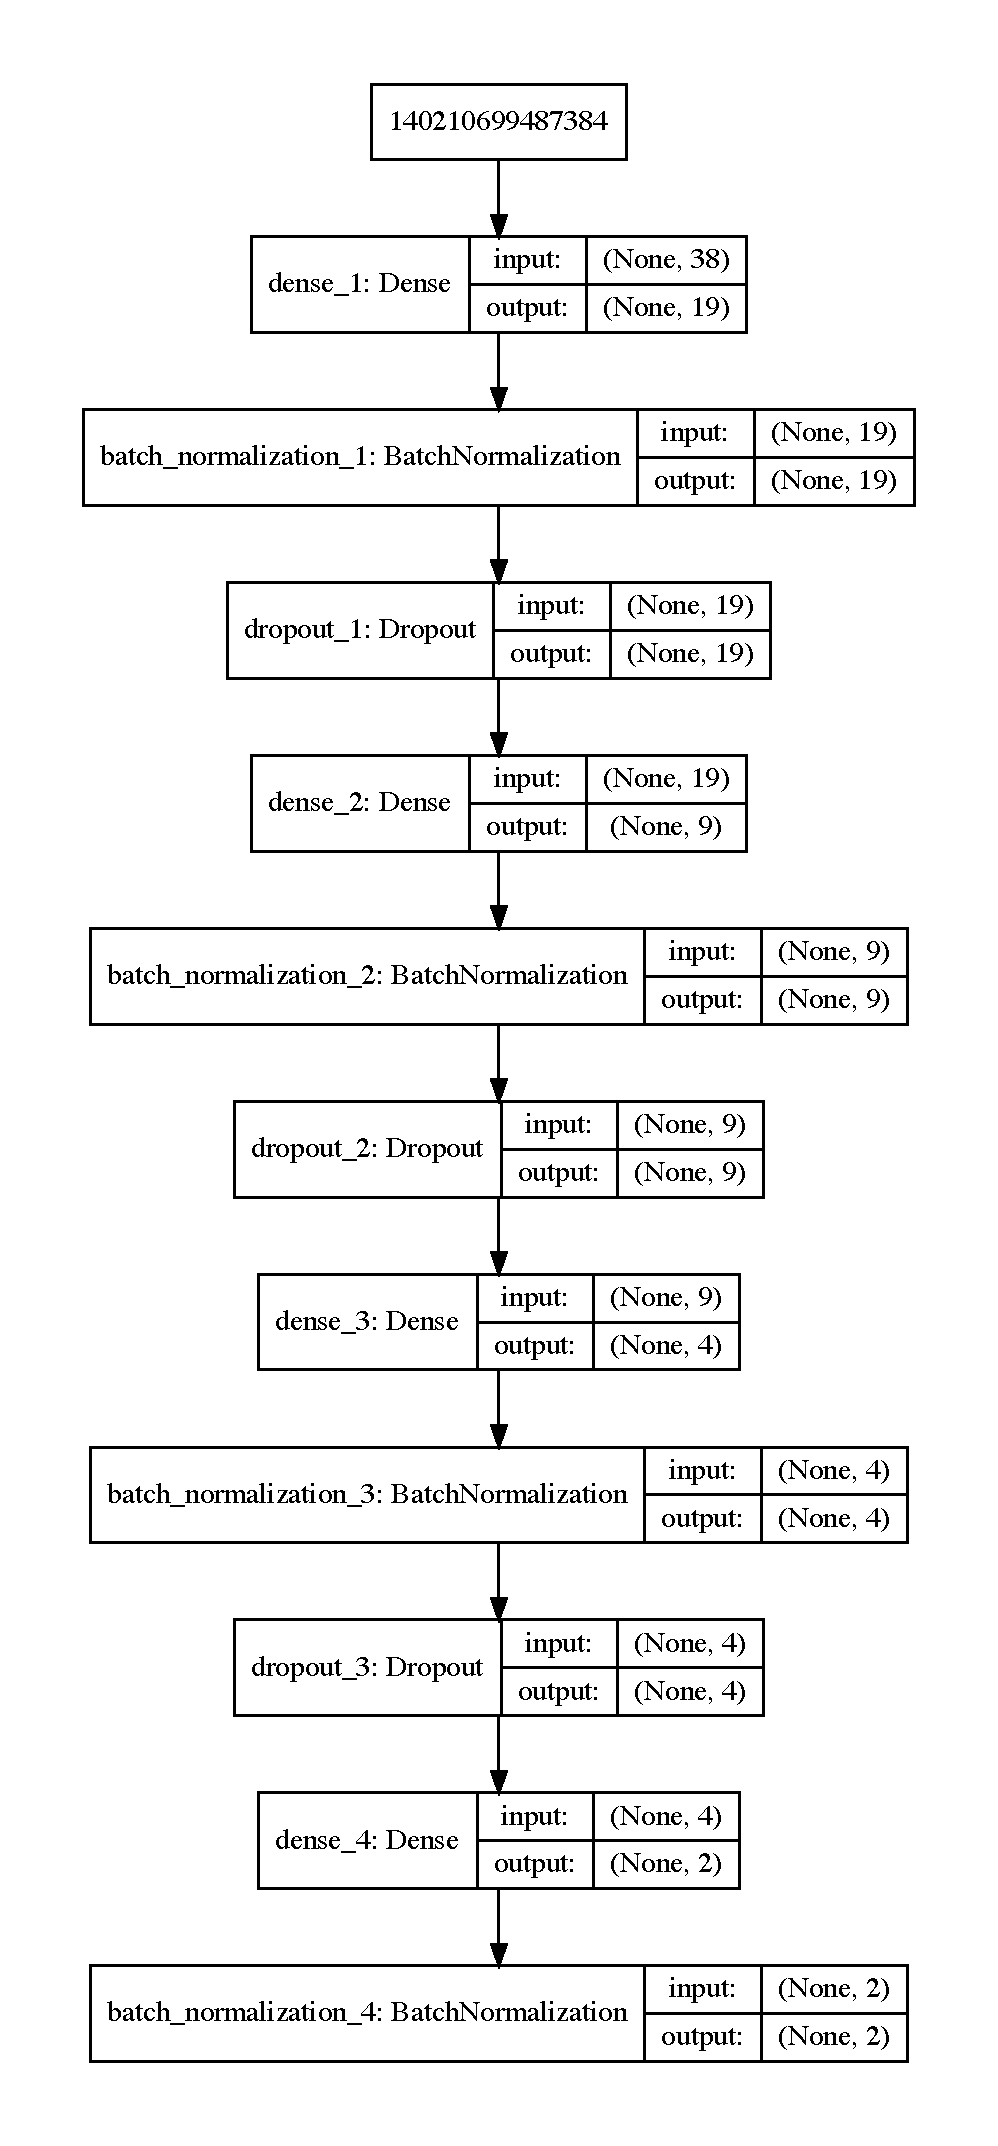
\includegraphics[scale=0.6]{./images/model_ae.pdf}
      \caption{\label{fig_ae}Autoencoder Architecture. }
\end{figure}

\begin{figure}[ht!]
  \centering
  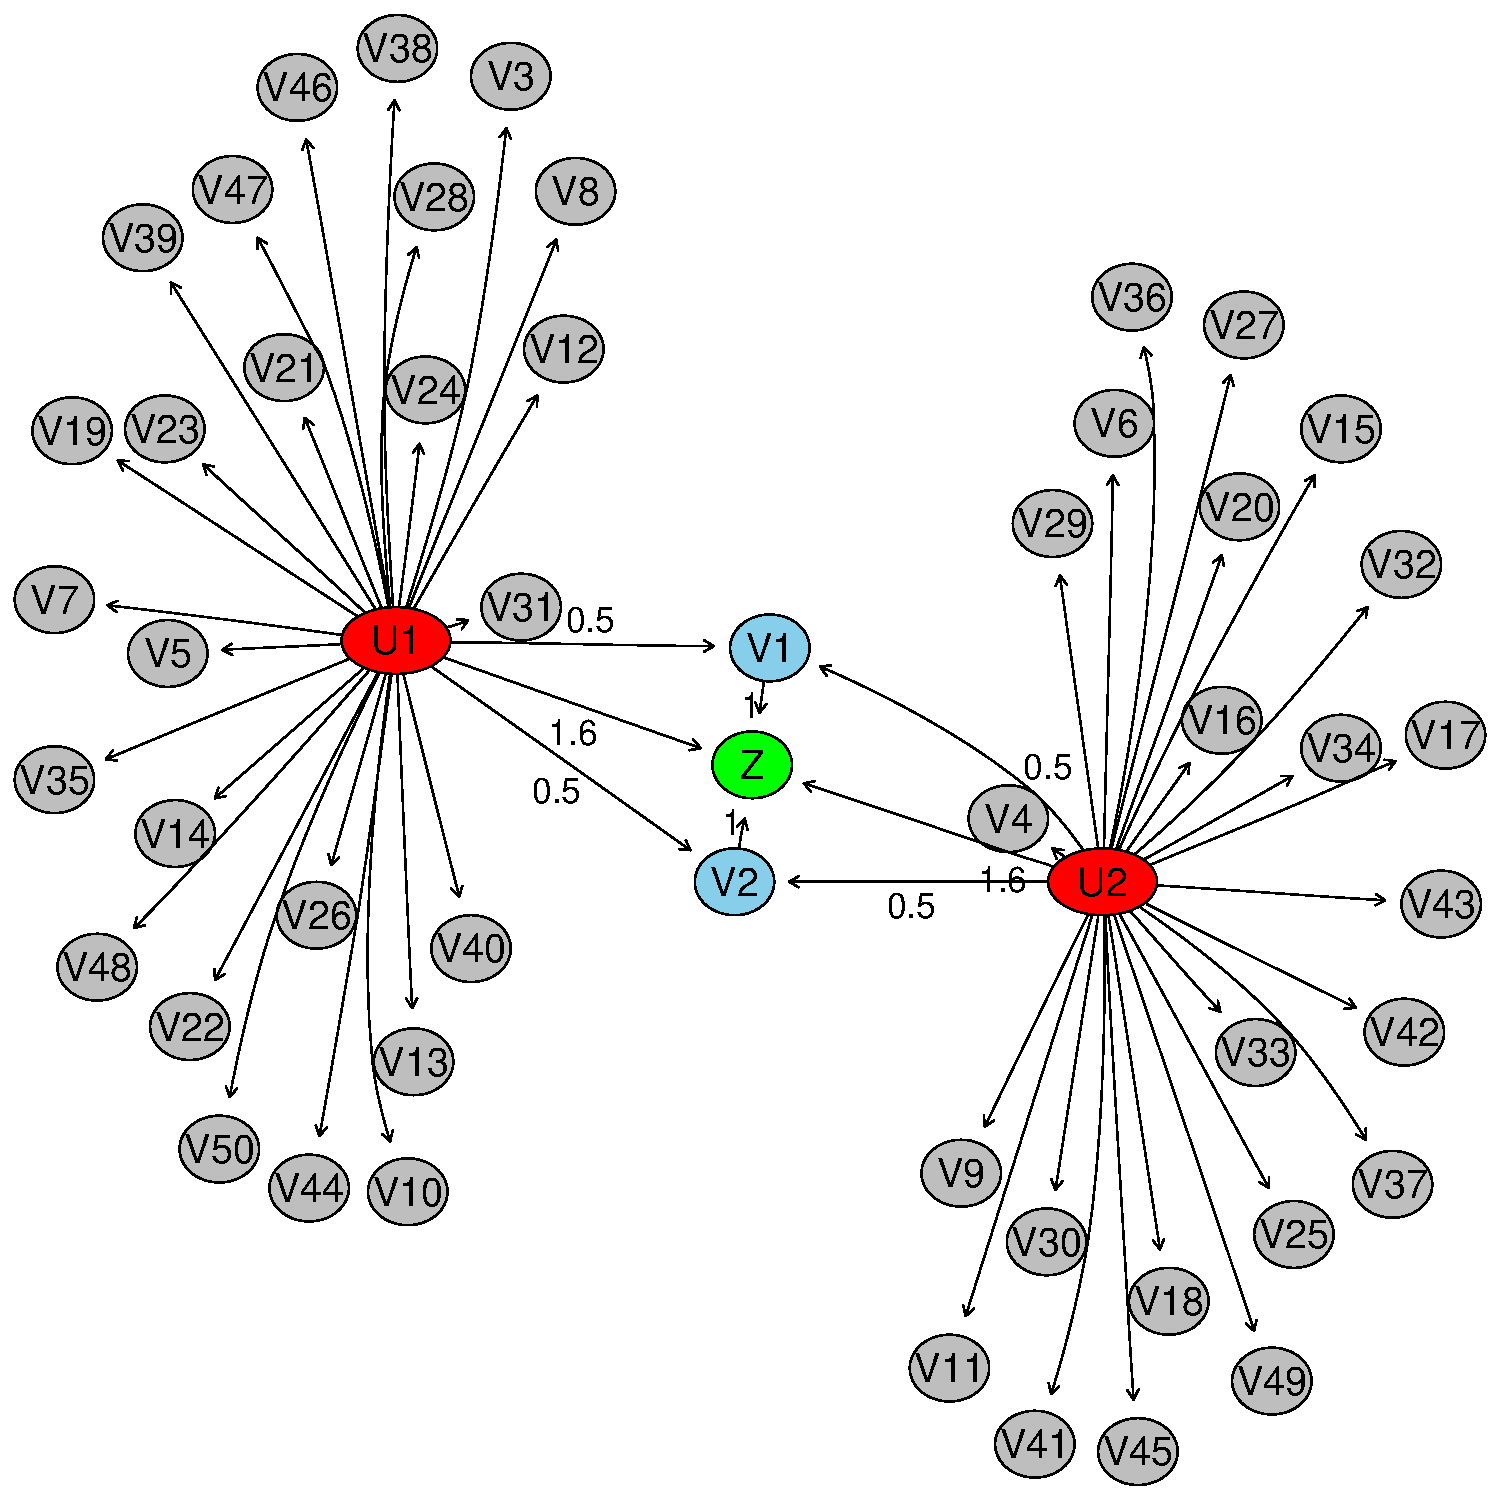
\includegraphics[width=\linewidth]{./images/true_network.pdf}
      \caption{\label{fig_network_true}True network. }
\end{figure}
\begin{figure}[ht!]
  \centering
  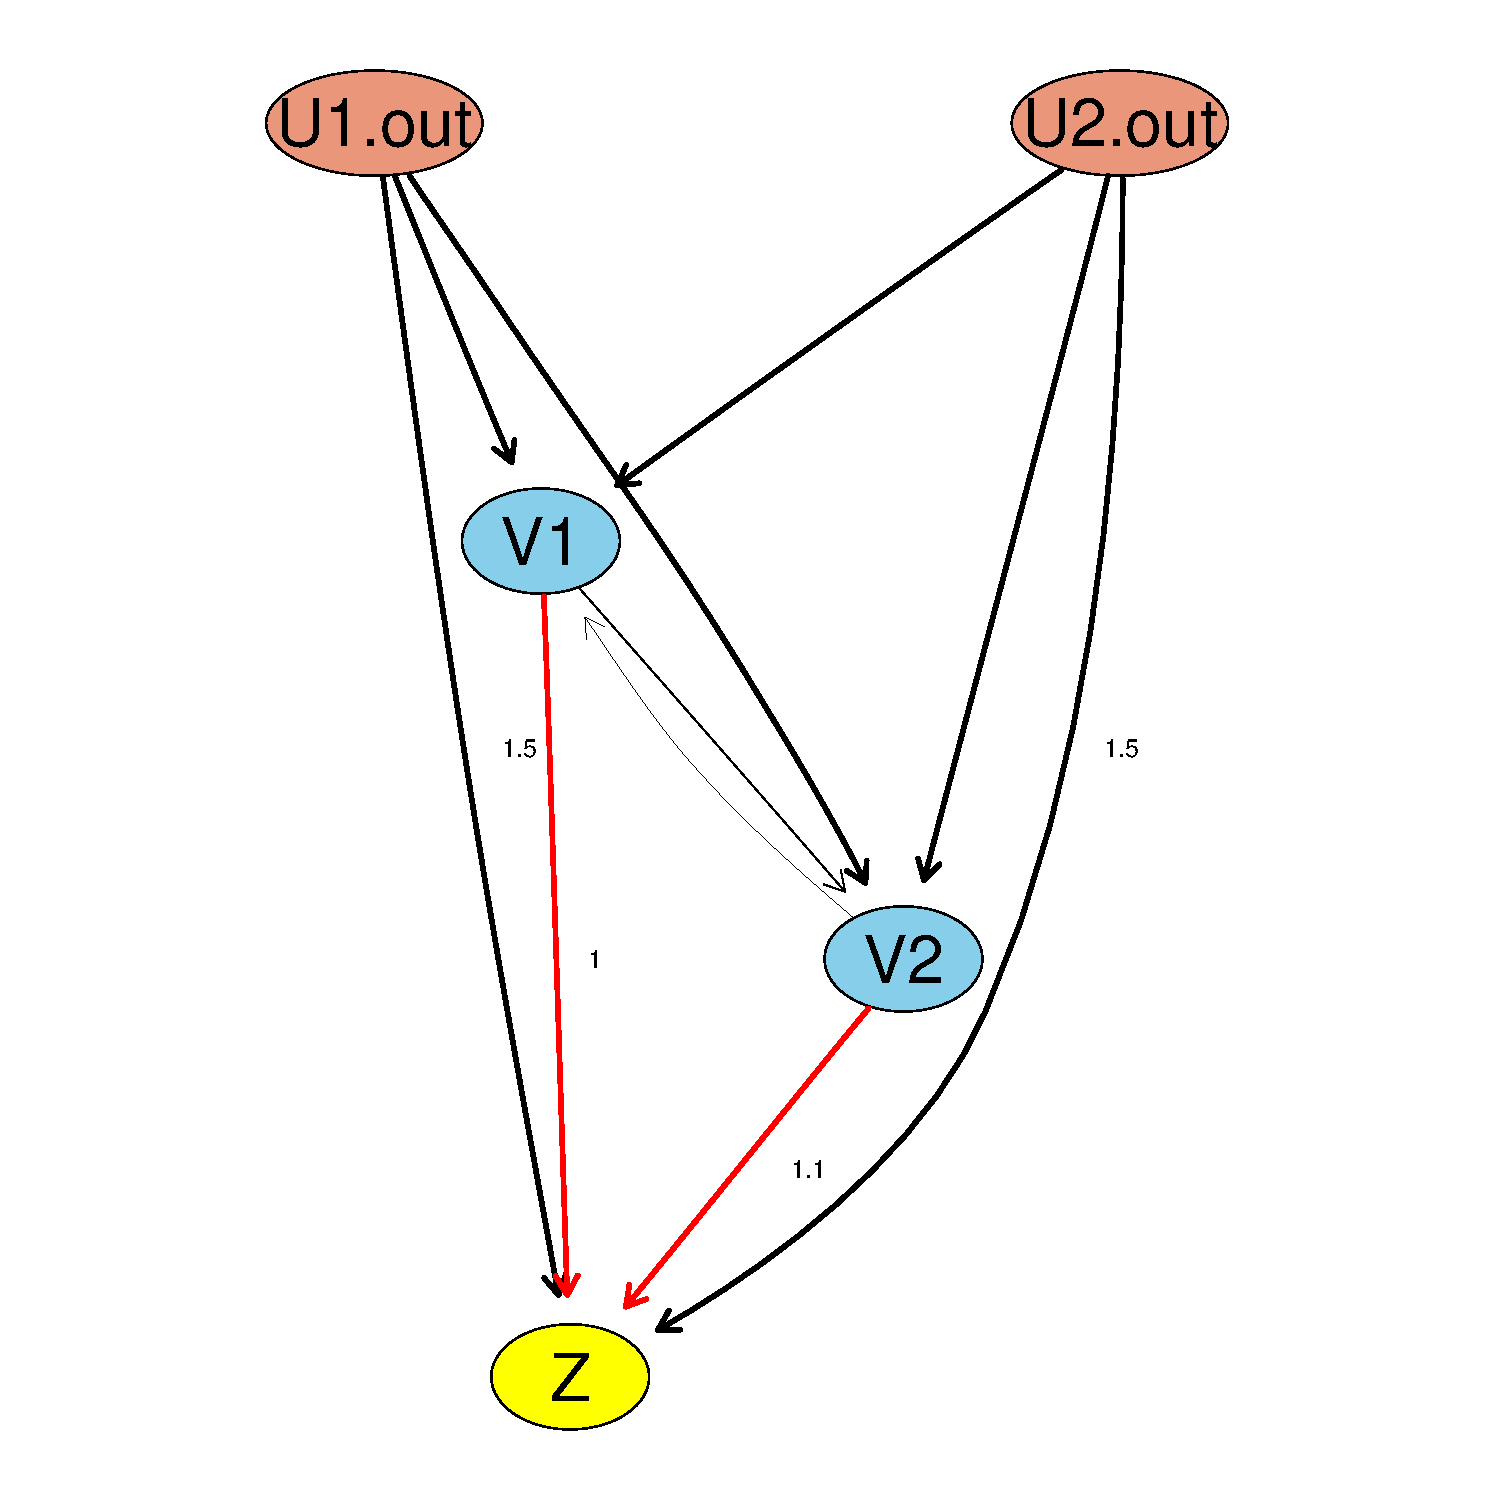
\includegraphics[width=\linewidth]{./images/estimated_network_fulldata.pdf}
      \caption{\label{fig_network_full}Infered network with complete dataset. }
\end{figure}

\begin{figure}[ht!]
  \centering
  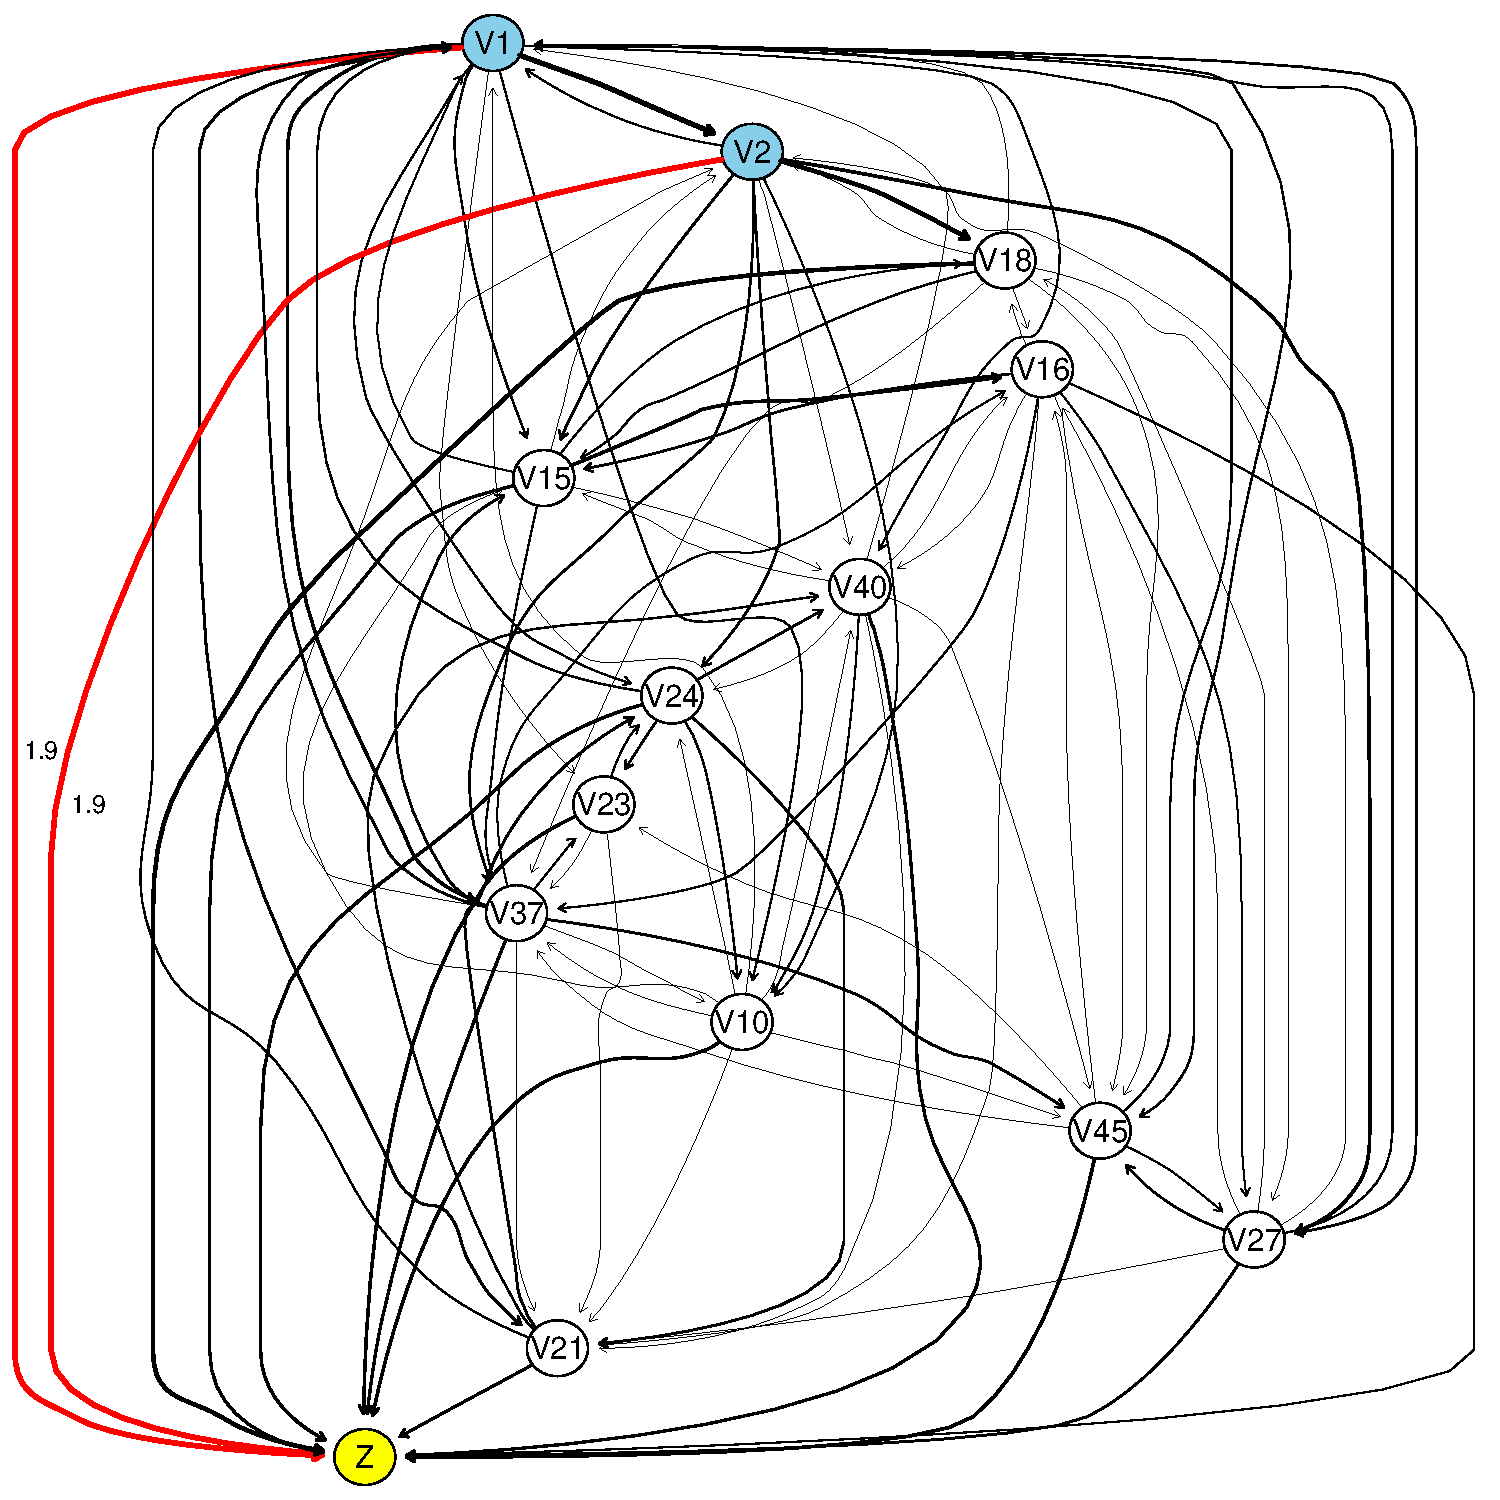
\includegraphics[width=\linewidth]{./images/estimated_network_missingdata.pdf}
      \caption{\label{fig_network_miss}Infered network when $U_1$ and
      $U_2$ are unobserved. }
\end{figure}


\begin{figure}[ht!]
  \centering
  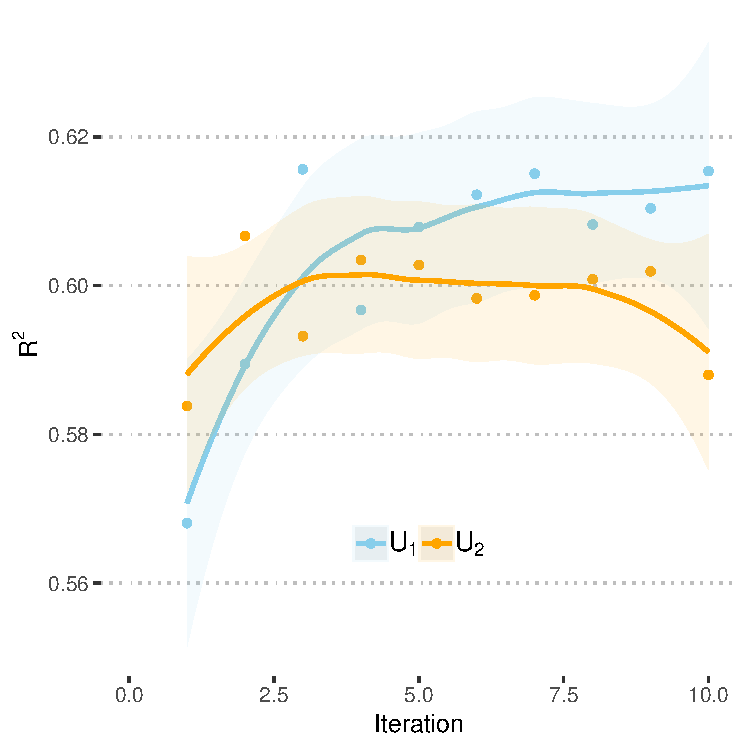
\includegraphics[width=\linewidth]{./images/fig_paper_r2lat.pdf}
      \caption{\label{fig_latvar_r2} $R^2$ in the prediction of the latent variable from the selected principal components}
\end{figure}

\begin{figure}[ht!]
  \centering
  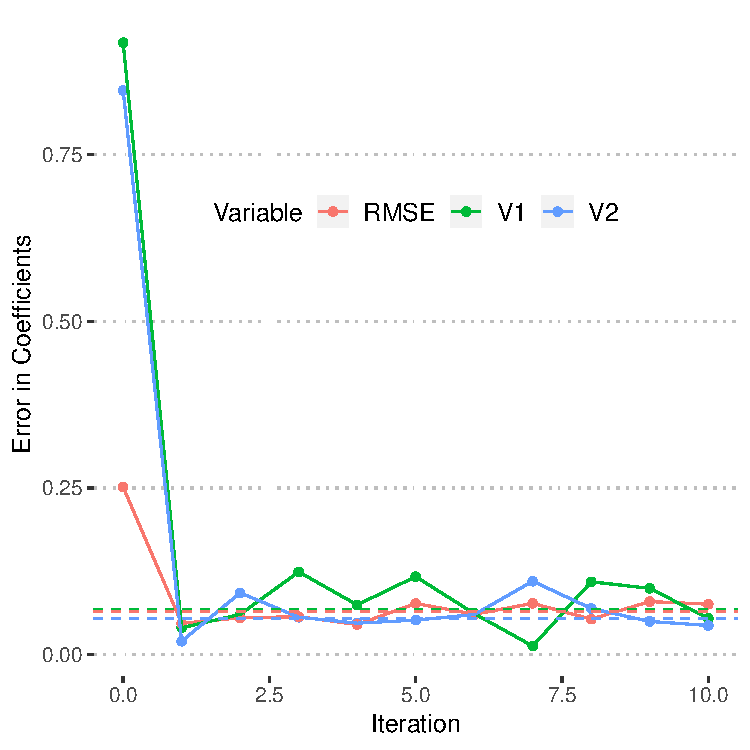
\includegraphics[width=\linewidth]{./images/fig_paper_errors.pdf}
      \caption{\label{fig_coef_rmse} Error in coefficients as a function of the iterations.}
\end{figure}


\begin{figure}[ht!]
  \centering
  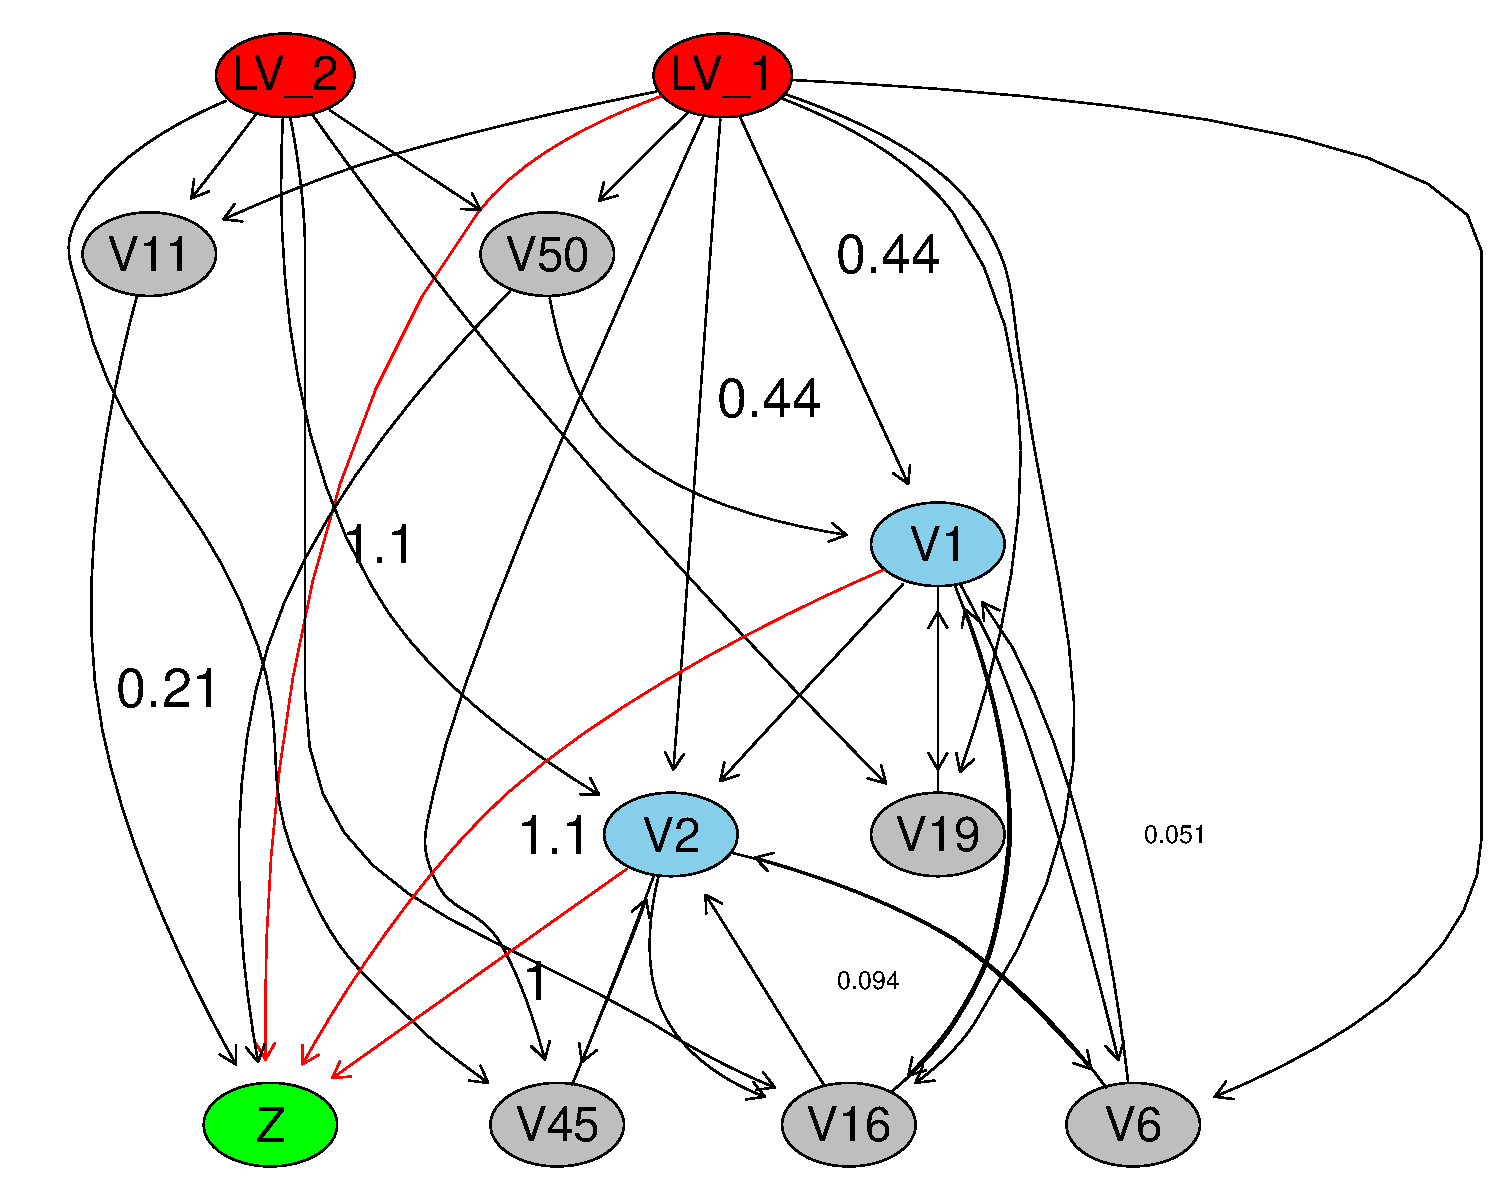
\includegraphics[width=\linewidth]{./images/estimated_network_infered.pdf}
      \caption{\label{fig_network_learn}Infered network at the last
      iteration of algorithm. }
\end{figure}

\begin{figure}[ht!]
  \centering
  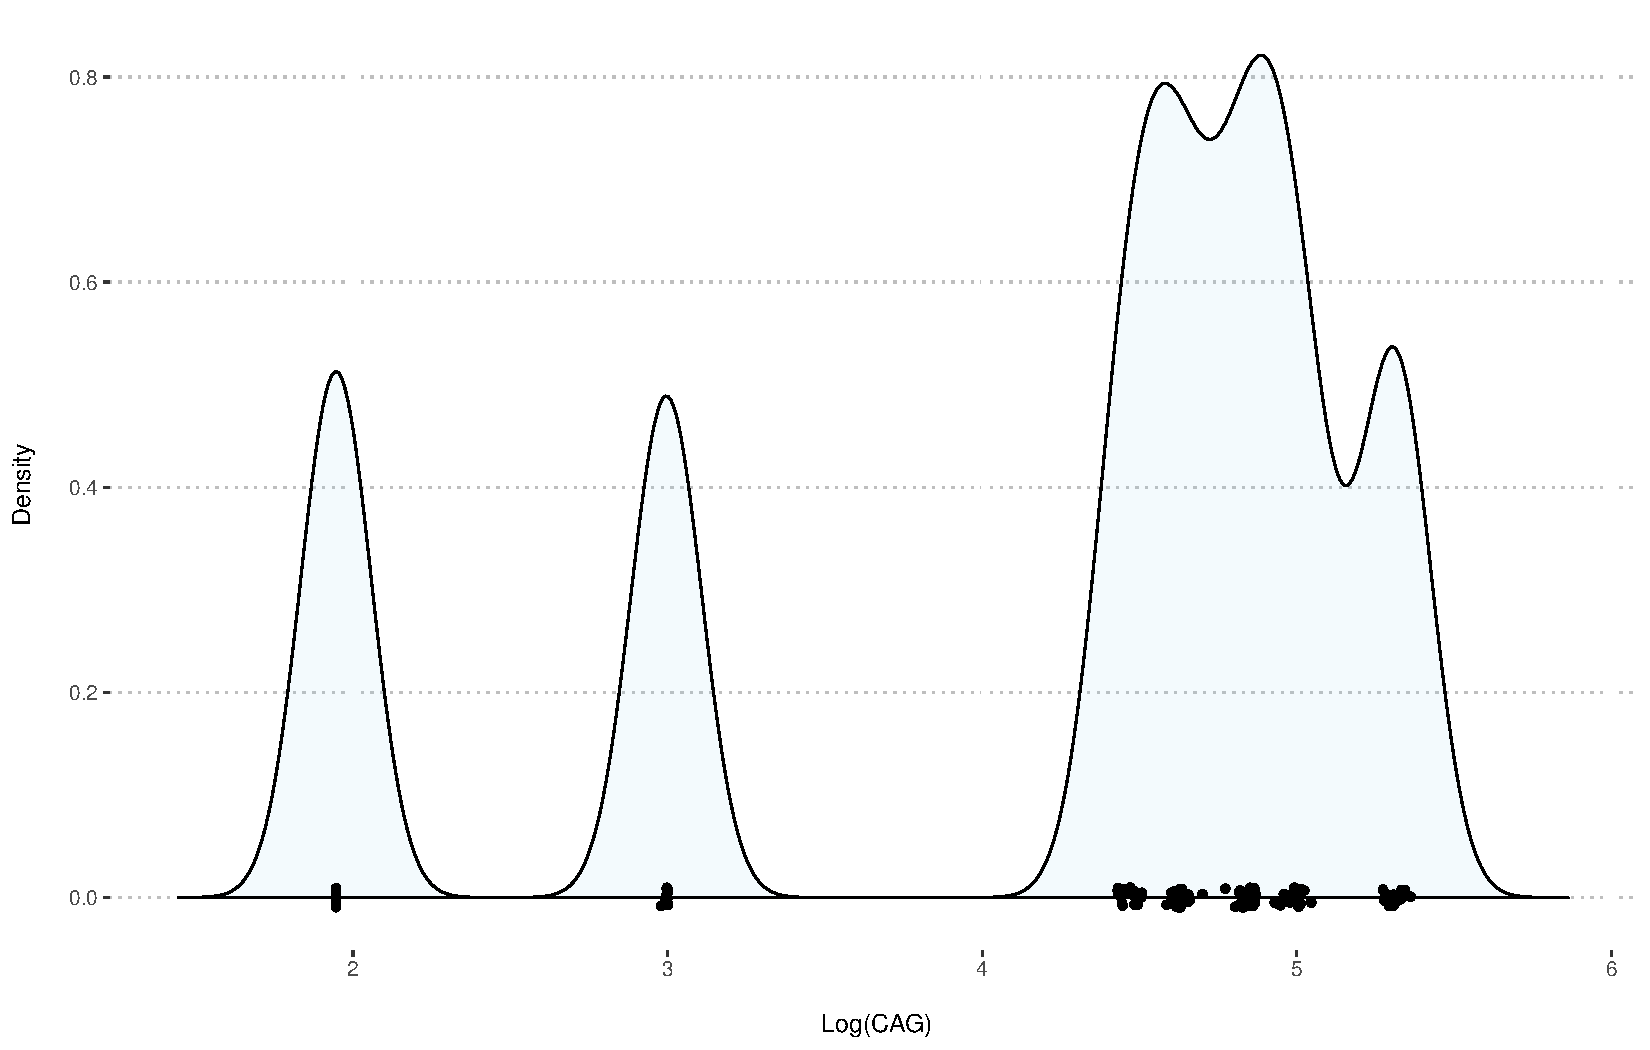
\includegraphics[width=\linewidth]{./images/cagPlots.pdf}
      \caption{\label{fig_cag_density} Density distribution of CAG. }
\end{figure}

\clearpage
\section{Additional Algorithms}
In this section we include additional algorithms

\begin{algorithm}%[H]
 \caption{Assesment Of Inference Of Latent CAG Repeat Length}
 \label{alg_cag}
\begin{algorithmic}
\State {\bfseries Data:} The CAG dataset, with CAG repeat length withheld
\State \textbf{Result:} Latent space predictive of CAG in training data and code to predict out of sample
 \For{fold $in$ 5 folds} 
  \State Train on 4/5 of the data
  \State Learn latent variables (linear, autoencoder methods)
  \State Predict out of sample
 \EndFor
 \State Concatenate all out-of-sample predictions across folds
 \State Assess $R^{2}$ for linear and autoencoder methods
\end{algorithmic}
\end{algorithm}

\section{Additional Examples}
\begin{figure}[ht!]
  \centering
  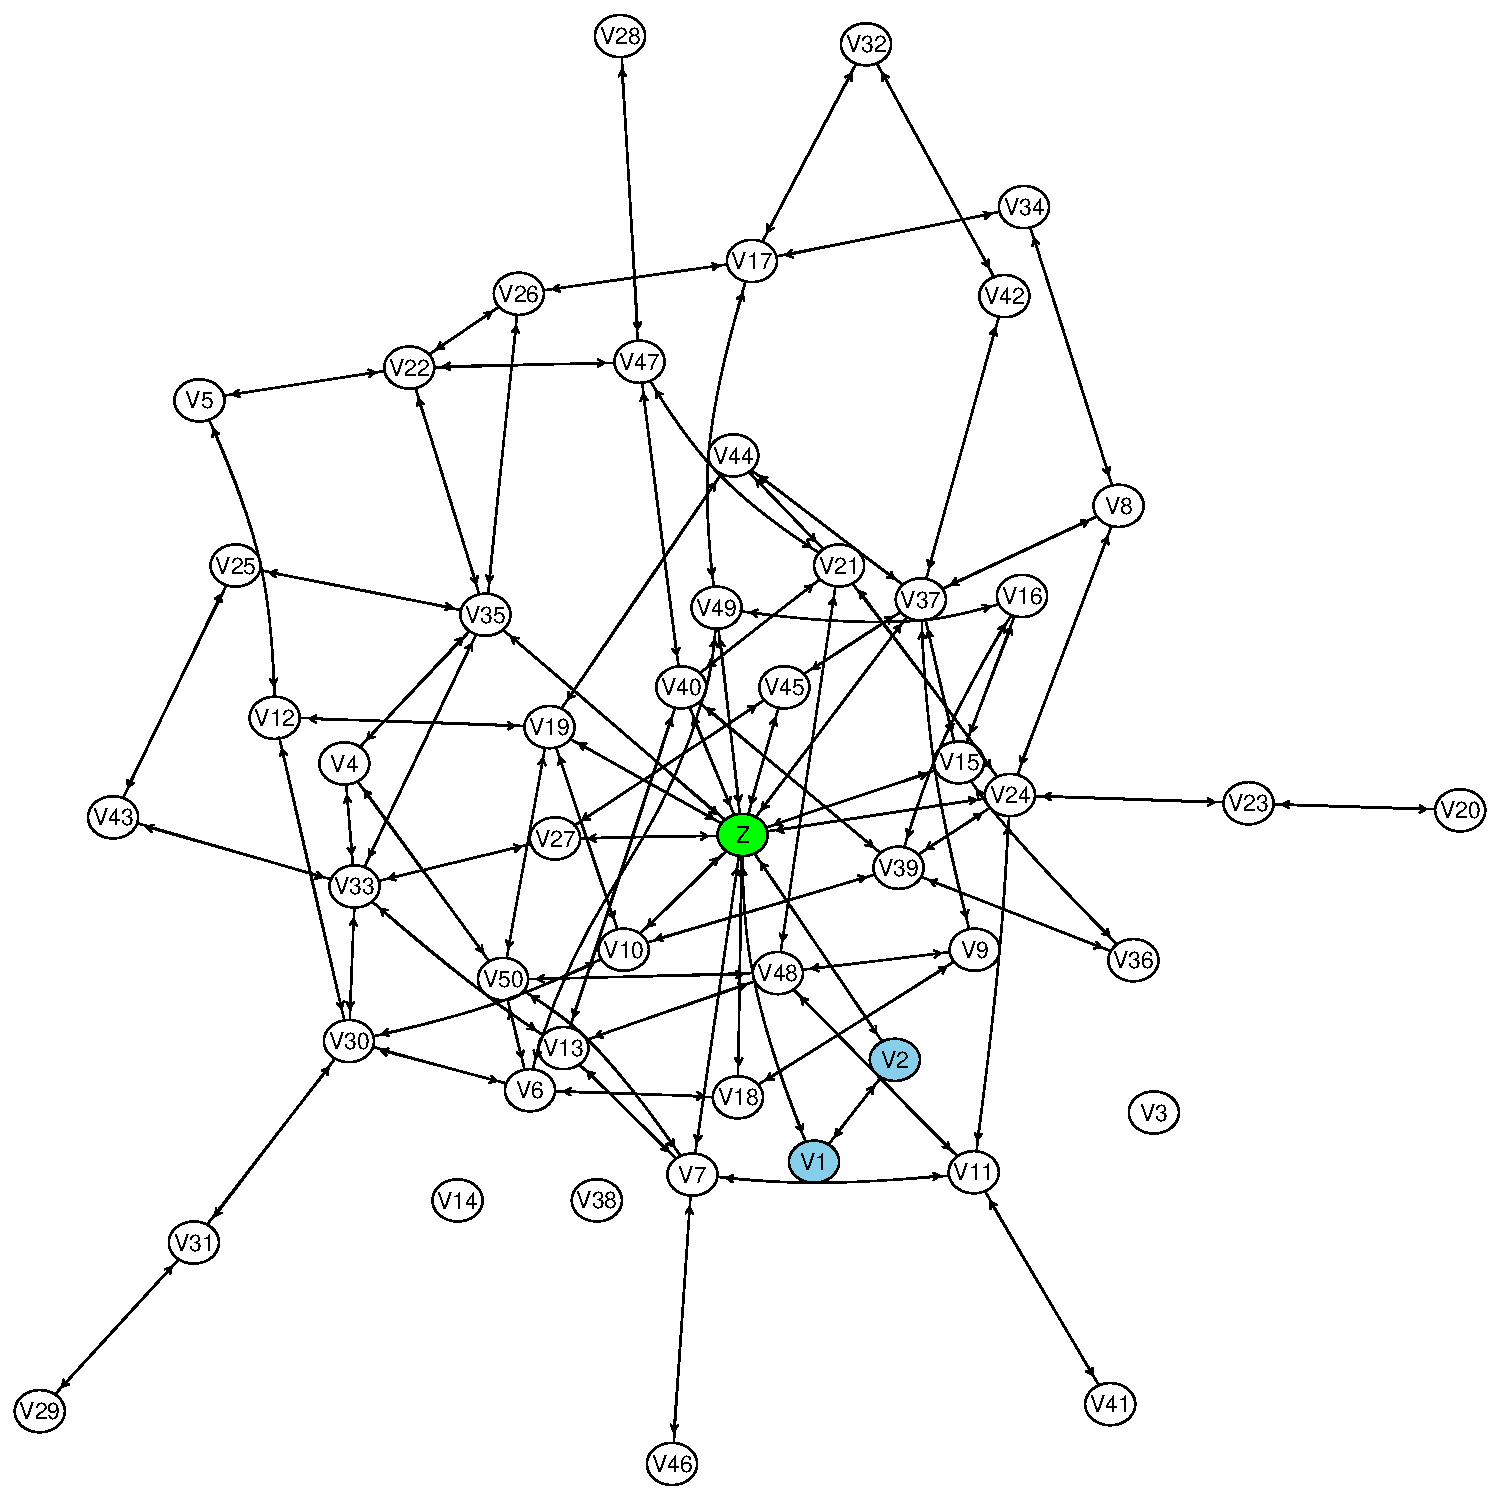
\includegraphics[width=\linewidth]{./images/rfcinet.pdf}
      \caption{\label{fig_rfci_ex1} RFCI reconstruction of synthetic
        example using CompareCausalNetworks R package.}
\end{figure}


\small
\bibliography{LatentVars-aaai}

\end{document}
